% !TeX root = ../main.tex
\documentclass[./../main.tex]{subfiles}

\begin{document}

\subsection{Mô hình ca sử dụng}

\subsubsection{Sơ đồ chính}

Hình \ref{fig:use_case_diagram} mô tả tác nhân và ca sử dụng chính của hệ thống.

\begin{figure}[h!]
  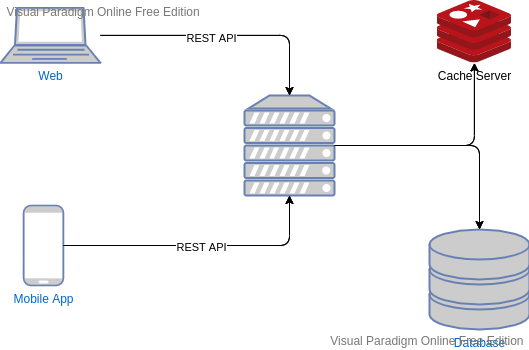
\includegraphics[width=\linewidth]{./images/image4.png}
  \caption{Mô hình ca sử dụng}
  \label{fig:use_case_diagram}
\end{figure}

\subsubsection{Tác nhân của hệ thống}

\begin{itemize}
  \item
    \begin{quote}
    \textbf{Người dùng} là người đã có tài khoản để truy cập vào hệ thống.
    \end{quote}
  \item
    \begin{quote}
    \textbf{Sinh viên} là người dùng hệ thống, sử dụng hệ thống để đăng ký
    thực tập, nộp báo cáo và xem kết quả thực tập.
    \end{quote}
  \item
    \begin{quote}
    \textbf{Giảng viên} là người dùng hệ thống, sử dụng hệ thống để quản
    lý và chấm điểm cho danh sách sinh viên đang hướng dẫn.
    \end{quote}
  \item
    \begin{quote}
    \textbf{Đối tác} là người dùng hệ thống, sử dụng hệ thống để quản lý
    bài đăng tuyển dụng, danh sách yêu cầu thực tập và danh sách sinh viên
    đang thực tập tại đơn vị.
    \end{quote}
  \item
    \begin{quote}
    \textbf{Quản trị viên Khoa} là người dùng hệ thống, sử dụng hệ thống
    để quản lý danh sách các kỳ thực tập, danh sách sinh viên, đơn vị thực
    tập, giảng viên theo từng kỳ và thông tin cá nhân của các đối tượng
    đó.
    \end{quote}
  \item
    \begin{quote}
    \textbf{Quản trị viên} là người dùng hệ thống, sử dụng hệ thống để
    quản lý danh sách các Khoa, danh sách lớp và quản lý tài khoản người
    dùng hệ thống.
    \end{quote}
  \end{itemize}

\end{document}